% arara: xelatex
% arara: xelatex
% arara: xelatex

% options:
% thesis=B bachelor's thesis
% thesis=M master's thesis
% czech thesis in Czech language
% english thesis in English language
% hidelinks remove colour boxes around hyperlinks

\documentclass[thesis=M,english]{prefs/FITthesis}[2019/03/06]

% \usepackage{subfig} %subfigures
% \usepackage{amsmath} %advanced maths
% \usepackage{amssymb} %additional math symbols

\usepackage[utf8]{inputenc}

\usepackage{graphicx} %graphics files inclusion
% \usepackage{amsmath} %advanced maths
% \usepackage{amssymb} %additional math symbols

\usepackage{dirtree} %directory tree visualisation
\usepackage{subfig} %image side by side
\usepackage{todonotes} %todo
\usepackage{url}
\usepackage{textcomp} %degree symbol
\usepackage{color, colortbl} %color, table color
\usepackage{enumitem} %lists
\usepackage{float} %for H option in figures
\usepackage{array} %table aligment       
\usepackage{amsmath} %cases
\usepackage{svg} %svg
\usepackage{scrextend}
\usepackage{multirow}
\addtokomafont{labelinglabel}{\sffamily}


% list of acronyms
\usepackage[acronym,nonumberlist,toc,numberedsection=autolabel,nomain]{glossaries}
% \iflanguage{czech}{\renewcommand*{\acronymname}{Seznam pou{\v z}it{\' y}ch zkratek}}{}
% \makeglossaries

\newcommand{\tg}{\mathop{\mathrm{tg}}} %cesky tangens
\newcommand{\cotg}{\mathop{\mathrm{cotg}}} %cesky cotangens

% % % % % % % % % % % % % % % % % % % % % % % % % % % % % % % % % % % 
% % % % % % % % % % % % % % % % % % % % % % % % % % % % % % % % % % % 
\department{Department of Applied Mathematics}
\title{People detection, tracking and biometric data extraction using a single camera for retail
usage}
\authorGN{Luk{\' a}{\v s}} %author's given name/names
\authorFN{Brchl} %author's surname
\authorWithDegrees{Bc. Luk{\' a}{\v s} Brchl} %author's name with academic degrees
\author{Luk{\' a}{\v s} Brchl} %author's name without academic degrees
\supervisor{doc. RNDr. Ing. Marcel Jiřina, Ph.D.}
\acknowledgements{}
\abstractCS{}
\abstractEN{}
\placeForDeclarationOfAuthenticity{} %where you have signed the declaration
\keywordsCS{}
\keywordsEN{.}
\declarationOfAuthenticityOption{5} %select as appropriate, according to the desired license
\website{https://github.com/lukasbrchl/People-detection-tracking-and-biometrics-extraction-using-a-single-camera-text} %optional URL (remove entirely if you have no URL for this thesis)

\begin{document}

\begin{introduction}
    Detection of people and their subsequent identity preservation in a video sequence (tracking) is a part of a more broader domain task called \gls{mot}. In the basic definition, \gls{mot} tries to estimate the position of the objects from multiple predefined classes, and then maintain their identity through the whole video sequence. 
    
    In most cases, position estimation is done by a component known as the object detector, which predicts the bounding boxes with real-valued confidences of each object class in each video frame. However, the conventional object detector does not guarantee the relationship between objects in consecutive frames. Therefore, it is necessary to extract additional features from each detected object to build the relationship in the sequence of frames. 
    
    The extracted features are mainly based on a visual appearance, movement, and interactions of the object, but complementary information such as camera calibration and known scene parameters can also be incorporated. The subsequent tracking is then achieved by matching detected objects to preserved tracks based on various distance metrics that are calculated between features of the detected objects in a current frame and features of traced objects from previous frames. This approach is also known as online tracking-by-detection which means that only current and previous frame information is available to the tracker, in contrast with offline-based tracking where information from the whole sequence can be used at any time. 
    
    One of the tracking benefits is that we can recover the trajectories of the objects that appeared in the video sequence, based on which we can calculate various spatial statistics that can help us to improve existing processes. For example, statistics about the movement within waiting halls might be helpful for companies to improve their indoor space and arrangement. 
    
    Even though this thesis focuses only on the task of people tracking, we may still apply many principles from more general \gls{mot}. A follow-up step after successfully building the people tracking framework is the extraction of additional class-specific information about people (soft-biometrics). This estimated data can be utilized in many applications from the retail environment; for example, we can utilize them in a retail store where there is the high demand for learning customer trends in specific days and hours, which could be easily achieved by collecting customer information such as age, gender, mood, etc. Other scenarios could be with a personalized advertisement targeted at passers-by in a shopping center or real-time staff alert when senior enters a store to offer immediate assistance. Moreover, we could use this framework to distinguish between customers and employees so we can analyze their interaction or even go further and optimize the distribution of employees around the store.
    
    \section{Motivation}
        \gls{mot} is one of the essential topics in the computer vision field. A large number of surveillance cameras in use has led to strong demand for automatic methods of processing their outputs. For example in the field of crowd image analysis, the scientific challenge is to devise and implement methods for obtaining detailed information about the number, density, movements, and actions involving people observed by a single camera or by a network of cameras.  
        
        Historically, the progress in \gls{mot} field has been limited by the number and size of the available datasets, and it was especially challenging to make comparisons between algorithms if they have been tested on different datasets under widely varying conditions. Thus, the needs of the researchers eventually formed the very first and most known PETS2009 \cite{ferryman2009pets2009} person tracking dataset. However, this dataset is minimalist. There are only three sequences related to the person tracking with ground-truth information, and evaluation metrics were often applied inconsistently, for example involving using different subsets of the available data, different ways of training the models, or differing evaluation scripts \cite{MOTChallenge2015}.
        
        The big break came in the year 2015 when MOTChallenge \cite{MOTChallenge2015} was released with the goal of standardization of quantitative benchmark to address such issues. Not only did they create unified evaluation framework with standardized metrics, but they also created the large-scale dataset with a total of 22 sequences, half for training and a half for testing purpose, with a total of 11286 frames or 996 seconds of video. This benchmark has massively transformed the \gls{mot} field which resulted in severe improvements to existing algorithms. Its popularity can also be expressed in numbers; for example, 99 \gls{mot} tracking algorithms were submitted to the MOT17 challenge \cite{mot16} during the year 2017 and similarly previous years. 
        
        Since the accuracy of existing algorithms is increasing and the price of \gls{gpu} computations is decreasing, new and more challenging datasets are being invented. VisDrone2018 \cite{zhuvisdrone2018} is a current state-of-the-art \gls{mot} dataset with over 260 video clips and more than 2.5 million bounding boxes of various class objects annotated. The frames are captured by several drone-mounted cameras which causes an unusual perspective and makes the dataset even more challenging. 
        
        To this date, there are more than ten large-scale \gls{mot} benchmarks publicly available which demonstrates that this task, especially with objects such as people, vehicles, and bicycles, has enormous attention in the research community and because the datasets are still updated to be more challenging, there are still places to improve. 
        
        The logical extension beyond detection and tracking horizons is the extraction of additional class-specific features. If we would track cars, we could take advantage of estimation of car paint, brand, and type. This information can then be used for various temporal and regional statistics; for example, for estimating the richness of a town by counting luxury-type cars. 
        
        If we take another case, which is the extraction of class-specific features about people, we could estimate attributes such as race, gender, height, mood, hair color, and clothes color. These traits are called soft-biometrics, and they are frequently used in cases where we need to complement primary biometric identifiers, such as fingerprint, palm veins, iris pattern, to provide authentication based on the unique identification of the person. The estimation of any class-specific feature is noisy. Therefore, it is essential to have reliable \gls{mot} framework, so the features are not collected from a single frame, but appropriately calculated from the whole tracking session.
        
        Although soft-biometric characteristics lack the distinctiveness and permanence to recognize an individual uniquely and reliably and can be easily faked, they provide some evidence about the people identity that could be beneficial \cite{wiki:biometrics}. With the use of soft-biometrics, we can differentiate individuals in surveillance video where it is ubiquitous that people are often occluded. In other words, despite the fact they are unable to individualize a subject, they are useful in distinguishing between people, thus maintaining people's identity in a surveillance scene. Another useful utilization is in the retail environment where we can build aggregated statistics such as the number of women between age 25 and 40 visited our store in the morning. If we have such information that in the morning there is 75 \% women of visitors, we could utilize this and adapt the store to be more suitable for women, and therefore we will have a better chance to increase profit.
        
        Last but not least, having an accurate and flawless \gls{mot} framework is crucial for further expansion to popular \gls{mtmct} field, which is the problem of determining who is where at all times given a set of video streams as input. The output of this task is also a set of person trajectories but from a wider area. Person \gls{reid} is a closely related problem in this field. Given a query image of a person, the goal is to retrieve from a database of images taken by different cameras the images where the same person appears. \cite{ristani2016MTMC}
        
    \section{Challenges}
        \gls{mot} field is deeply explored -- many methods have been proposed, and many surveys have been conducted \cite{luo2014multiple, fan2016survey, emami2018machine}. However, it is still considered as not successfully solved computer vision task. In other words, a saturation point has not yet been reached.
        
        \gls{mot} task is an extension of object detection from single images to video sequence. 
        The main challenges when using an object detector for tracking are that the resulting output is unreliable and sparse, i.e., detectors only deliver a discrete set of responses and usually yield false positives and false negatives (missing detections) as shown in Fig \ref{fig:false positive and false negative}. So, in addition to such object detection errors, identity switches are frequent in any \gls{mot} framework (see Fig. \ref{fig:id switch example}). 
    
        \begin{figure}[ht]
          \centering
          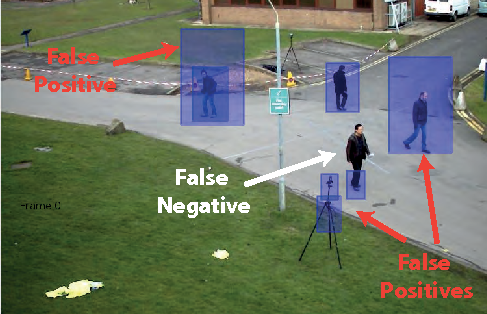
\includegraphics[width=0.7\textwidth]{resources/false-positive_and_false_negative.png}
          \caption{Example of false positive and false negative person detection. Source: \cite{yao2012interactive}.}
          \label{fig:false positive and false negative}
        \end{figure}
        
        \begin{figure}[ht]
          \centering
          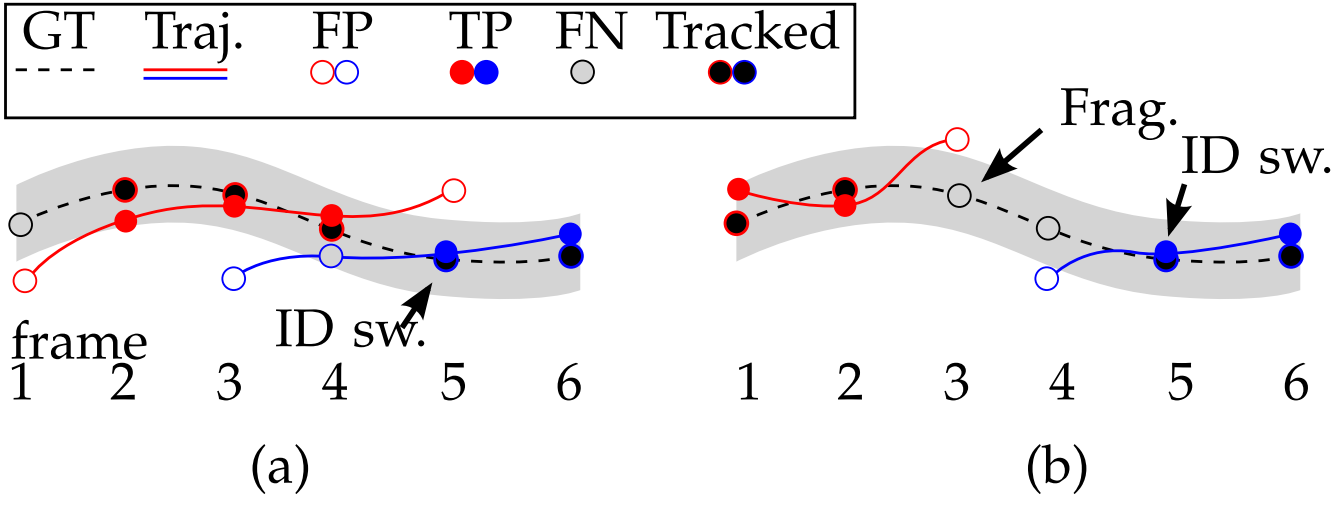
\includegraphics[width=0.7\textwidth]{resources/tracking_errors.png}
          \caption{Cases illustrating tracker-to-target assignments errors. (a) An ID switch occurs when the mapping switches from the previously assigned red track to the blue one. (b) A track fragmentation is counted in frame 3 because the target is tracked in frames 1 and 2, then interrupts, and then reacquires its ‘tracked’ status at a later point. A new (blue) track hypothesis also causes an ID switch at this point. Source: \cite{MOTChallenge2015}}
          \label{fig:id switch example}
        \end{figure}
        
        ID switches occur when there are two object trajectories are produced for one ground-truth object. Fragmentation occurs when there are two trajectories are produced with a time gap between them for one ground truth object, which implies that detections are missed in several frames. In theory, the robust tracker should handle both of these flaws. It should fill gaps in detections by propagating information from neighboring frames, and it should also filter false positive detections based on the information from previous frames. 
        
        However, it has been found out during multiple object tracking challenges that in practice, it is not entirely so. For example, in \gls{mot} \cite{mot16} dataset from 2016, 18 \% of tracks are not covered by detections at all, and 37 \% percent of tracks are covered only by low confidence of detections. When there is no high-quality detection for particular ground-truth track, then the tracker cannot resolve this problem at all, which implies that tracker usually reduces only false positives and raise false negatives by removing low-confidence detections. Nowadays, many researchers state that a robust object detector is a key to good tracking \cite{mot16, konushin2017, bewley2016simple} and during recent work \cite{luo2014multiple, fan2016survey, DBLP:journals/corr/abs-1903-05625}, it has been shown that modern object detectors can locate object even in complex, crowded scenes. However, false positives have remained frequent. 
        
        If we narrow down to the tracking people, it is even more difficult because they are very dynamic objects. People tend to change position, direction, and posture often, but they also have different height and body proportions. In real-world scenes, long-term occlusions are also frequent. As a result, it is vital for people tracking systems to be flexible so that it can handle as many different situations as possible.  
        
        Lastly, it is a topic from computer vision field where most of the work is done over images represented by matrices. It is well known that working with images is computationally demanding because each change needs to be applied for each pixel and although the image algorithms can be well parallelized, we still need to keep in mind the computation costs. 
    
    \section{Objectives}
        The goal of this thesis is to design and implement a sophisticated framework that could utilize surveillance sequences for people online tracking followed by the extraction of as much data as possible about the people in the scene, which is a three-step process. First, we need effectively and precisely acquire people detections in each frame. Then, we need to utilize a robust tracking algorithm that will maintain people identities. Lastly, gathered data from people tracking sessions must be appropriately processed for useful output statistics.
    
    \section{Assumptions}   
        The detection and tracking of people in surveillance footage is a broad topic. For this reason, the work is limited only to the one static camera watching a known scene. We assume that the captured scene is entirely under our control which means we can make any measurements and calibrate the camera. Moreover, we take into account the requirements for online processing so that the framework can be improved for real-time inference in the future. 
    
    \section{Thesis structure}
        The rest of this thesis is organized as follows. In the first chapter, we present a theoretical background which is crucial for the understanding of solving this task. Chapter 2 is devoted to the related work. Algorithm design and proposals are presented in chapter 3. Implementation details are explained in chapter 4, followed by the evaluation presented in chapter 5. The whole work is wrapped up in the last Conclusion chapter.
    
\end{introduction}
\chapter{Existing methods}
\chapter{Analysis}
\chapter{Design}
\chapter{Implementation}
    This chapter contains information related to the implementation of the proposed framework. The whole implementation is done in Python language with the dependence on several other frameworks and libraries, including OpenCV, Tensorflow, and Darknet. The main application functionality spans eight Python modules.
    
\section{Module tracking\textunderscore app}
    This module is the main entry point of the application. It contains only one essential function that is responsible for running the proposed framework. In this function, we first load the input image stream, calibration parameters and other components such as object detectors, feature extractors, tracker, and image viewer. Then there is a loop that runs the algorithms as long as input frames are available. The application can be run either from an IDE or from the command line with various input parameters.

\section{Module detection}
    The detection module contains multiple wrappers for various object and face detectors proposed in \ref{detection_and_tracking_components}. It is responsible for loading these models based on input parameters, detecting objects in the input frame, and filtering detections by input criteria. 

\section{Module feature\textunderscore extraction}
    In this module, we propose to interface and pre-processing to various appearance feature extractors including age, gender, and emotion models, but also height estimator. The module also contains a function that assigns face regions to people bounding boxes.

\section{Module kalman\textunderscore filter}
    This module is vital for the proposed motion analysis method because it contains the configuration of the utilized filter. Our approach uses Kalman Filter implementation from famous FilterPy \cite{labbe2015kalman} library. The module is also responsible for converting filter's internal state to visualizable bounding box and for converting measurements to filter's input.

\section{Module matching}
    The matching module contains an efficient implementation of a proposed distance metric, namely the cosine metric for appearance (section \ref{appearance_metric}) and enhanced Euclidean distance for the state (section \ref{state_metric}). Metrics are calculated by NumPy, which is a high-performance linear algebra library written in C language. To make the computations as efficient as possible, we utilize the NumPy broadcasting technique.

\section{Module tracking}
    In the tracking module, we propose PeopleTracker class that is responsible for the actual matching of detections and tracks. It is mostly inspired by code from \cite{wojke2017simple}, but some modifications in the matching algorithm were made. Successfully matched tracks are updated from here, and unmatched detections are transformed to tentative tracks.
    
\section{Module track}
    An instance of Person class from the track module represents a single person that was detected in the scene. Each person instance has set of attributes including id, color for visualization, status, creation frame number, time since the last update, age in frame units, last body bounding box, last face bounding box, Kalman filter instance, and dictionary with gathered features.
    
\section{Module output\textunderscore statistics}
    This module is responsible for transforming all possible data to brief output statistics. It includes a class TrackingEvaluator which evaluates the tracking performance of the algorithm based on provided annotations. Class OutputStatistics is responsible for converting gathered data about people to usable outputs.

\section{Module visualization}
    Visualization module contains all drawing related functions including plotting output graphs using Matplotlib and Seaborn libraries. It implements an ImageViewer class that is responsible for showing the preview of processed images. The ImageViewer class also contains functionality that allows easier debugging by allowing users to pause the algorithm or process the stream by one frame at a time.
\chapter{Evaluation}
%Further work
\begin{conclusion}
    This work was focused on building a framework for the task of people tracking and soft-biometric data extraction. In the introductory chapter, we thoroughly described the assignment with sufficient motivation, but also with its challenges. In the following theoretical chapter, we have described the necessary theoretical background in detail for understanding of this thesis. In chapter \ref{related_work}, we briefly reviewed the existing solutions, and based on that some popular methods were implemented from scratch or customized from open-source repositories to meet the thesis goals. The implemented solution is then evaluated in the evaluation chapter, and further improvements are proposed. The result is a functioning people tracking and soft-biometrics extracting framework that can be deployed in a real-world application.
    
    According to the table \ref{table:tracking_results}, the proposed algorithms achieve {state-of-the-art} results in long-term people tracking. The best solution based on \gls{faster r-cnn} achieves only two identity switches on our dataset, which is an outstanding outcome. The quality of the detected boxes is also very high. Evaluated height and age estimators achieve exact results. However, in future work, it is necessary to evaluate more individuals.
    
    The proposed methods are designed in several variations to meet different trade-offs of accuracy versus computational expensiveness, and since the final design of the framework is fully modular, it can be easily configured to meet demands for various other scenarios. We put much effort into the application design as a whole so that it can be easily expanded and it can now be deployed in real-world applications. There are still some shortcomings in the framework, but they are described so that they can be further worked on and we hope that this work will be a useful as a starting point for other people interested in this topic. 

\end{conclusion}

% bibliography
\bibliographystyle{prefs/iso690}
\bibliography{ref}

\appendix

% acronyms
% \newacronym{TST}{TST}{Test}
\printglossaries

% media contents
\chapter{Media contents}\label{app:CDcontent}
\begin{figure}
% 	\dirtree{%
% 		.1 readme.txt\DTcomment{the file with CD contents description}.
% 		.1 data\DTcomment{the data files directory}.
% 		.2 graphs\DTcomment{the directory of graphs of experiments}.
% 		.3 *.eps\DTcomment{the B/W graphs}.
% 		.3 *.png\DTcomment{the color graphs}.
% 		.3 *.dat\DTcomment{the graphs data files}.
% 		.1 exe\DTcomment{the directory with executable WBDCM program}.
% 		.2 wbdcm\DTcomment{the WBDCM program executable (UNIX)}.
% 		.2 wbdcm.exe\DTcomment{the WBDCM program executable (Windows)}.
% 		.1 src\DTcomment{the directory of source codes}.
% 		.2 wbdcm\DTcomment{the directory of WBDCM program}.
% 		.3 Makefile\DTcomment{the makefile of WBDCM program (UNIX)}.
% 		.2 thesis\DTcomment{the directory of \LaTeX{} source codes of the thesis}.
% 		.3 figures\DTcomment{the thesis figures directory}.
% 		.3 *.tex\DTcomment{the \LaTeX{} source code files of the thesis}.
% 		.1 text\DTcomment{the thesis text directory}.
% 		.2 thesis.pdf\DTcomment{the Diploma thesis in PDF format}.
% 		.2 thesis.ps\DTcomment{the Diploma thesis in PS format}.
% 	}
\end{figure}


\end{document}
